\documentclass[DM,lsstdraft,toc]{lsstdoc}

% lsstdoc documentation: https://lsst-texmf.lsst.io/lsstdoc.html

% Package imports go here.

% Local commands go here.

% To add a short-form title:
% \title[Short title]{Title}
\title{Data Management Database Design}

% Optional subtitle
% \setDocSubtitle{A subtitle}

\author{%
	Jacek Becla,
	Daniel Wang,
	Serge Monkewitz,
	K-T Lim,
	John Gates,
	Andy Salnikov,
	Andrew Hanushevsky,
	Douglas Smith,
	Bill Chickering,
	Michael Kelsey,
	and
	Fritz Mueller
}

\setDocRef{LDM-135}

\date{\today}

% Optional: name of the document's curator
% \setDocCurator{The Curator of this Document}

\setDocAbstract{%
This document discusses the LSST database system architecture.
}


% Change history defined here.
% Order: oldest first.
% Fields: VERSION, DATE, DESCRIPTION, OWNER NAME.
% See LPM-51 for version number policy.
\setDocChangeRecord{%
  \addtohist{1.0}{2009-06-15}{Initial version.}{Jacek Becla}
  \addtohist{2.0}{2011-07-12}{Most sections rewritten, added scalability test section}{Jacek Becla}
  \addtohist{2.1}{2011-08-12}{Refreshed future-plans and schedule of testing sections, added section about fault tolerance.}{Jacek Becla, Daniel Wang}
  \addtohist{3.0}{2013-08-02}{Synchronized with latest changes to the requirements \citedsp{LSE-163}. Rewrote most of the “Implementation” chapter. Documented new tests, refreshed all other chapters.}{Jacek Becla, Daniel Wang, Serge Monkewitz, Kian-Tat Lim, Douglas Smith, Bill Chickering}
  \addtohist{3.1}{2013-10-10}{Refreshed numbers based on latest \citeds{LDM-141}. Updated shared scans (implementation) and 300-node test sections, added section about shared scans demonstration}{Jacek Becla, Daniel Wang}
  \addtohist{3.2}{2013-10-10}{TCT approved}{R Almsman}
  \addtohist{}{2016-07-18}{Update with async query, shared scan, secondary index, XRootD, metadata service information.}{John Gates, Andy Salnikov, Andrew Hanushevsky, Michael Kelsey, Fritz Mueller}
  \addtohist{}{2017-07-05}{Move historical investigations to separate documents: \citeds{DMTN-046,DMTN-047,DMTN-048,DMTR-21,DMTR-12}}{T.~Jenness}
  \addtohist{}{2017-07-07}{Bring up to date with current status, condense requirements section, re-order sections for improved readability.}{Fritz~Mueller}
}

\begin{document}

% Create the title page.
% Table of contents is added automatically with the "toc" class option.
\maketitle

\section{Executive Summary}\label{executive-summary}

Two facets of LSST database architecture and their motivating requirements
are discussed: database architecture in support of real time Alert Production,
and database architecture in support of user query access to catalog data.
Following this, Qserv is explored in depth as an implementation of the query
access architecture.

The LSST baseline database architecture for real time Alert
Production relies on horizontal time-based partitioning. To guarantee
reproducibility, no-overwrite-update techniques combined with
maintaining validity time for appropriate rows are employed. Two
database replicas are maintained to isolate live production catalogs
from user queries; the replicas are synchronized in real time using
native database replication.

The LSST baseline database architecture for user query access to catalog data
is an MPP (massively parallel processing) relational database composed of a
single-node non-parallel DBMS, a distributed communications layer, and a
master controller, all running on a shared-nothing cluster of commodity
servers with locally attached spinning disk drives, capable of incremental
scaling and recovering from hardware failures without disrupting running
queries. All large catalogs are spatially partitioned horizontally into
materialized \emph{chunks}, and the remaining catalogs are replicated on each
server; the chunks are distributed across all nodes. The Object catalog is
further partitioned into \emph{sub-chunks} with overlaps, materialized on-the-
fly when needed. Chunking is handled automatically without exposure to users.
Selected tables are also partitioned vertically to maximize performance of
most common analysis. The system uses a few critical indexes to speed up
spatial searches, time series analysis, and simple but interactive queries.
Shared scans are used to answer all but the interactive queries. Such an
architecture is primarily driven by the variety and complexity of anticipated
queries, ranging from single object lookups to complex \(O(n^2)\) full-sky
correlations over billions of elements.

A prototype implementation of the baseline architecture for user query access
as described above, \emph{Qserv}, was developed during the R&D phase of LSST,
and its feasibility was demonstrated in early testing.  Productization was
subsequently planned and resourced for the construction phase of LSST and is
presently underway.

Qserv leverages two mature, open-source technologies as major components of
its design: MySQL as a SQL execution engine (though any alternative SQL engine
could be substituted without undue effort if need be), and
XRootD\footnote{\url{http://xrootd.org}} \citep{Dorigo:2005:XRootd} to provide
a distributed-system framework for fault-tolerant, elastic, content-addressed
messaging.

We currently maintain three running instances of Qserv at a scale of
approximately 30 physical nodes each in continuous operation on dedicated
hardware clusters at NCSA and CC-IN2P3. The system has been demonstrated to
correctly distribute and execute both low and high volume queries, including
small-area cone and object searches, region restricted queries, and full table
scans including large-area near-neighbor searches. Analytic queries involving
SciSQL UDFs in both filter and aggregation clauses have also been
demonstrated. Scale testing has been successfully conducted on the
above-mentioned clusters with datasets of up to approximately 70 TB, and we
expect to cross the 100 TB mark as tests continue in 2017. To date the system
is on track through a series of graduated data-challenge style tests to meet
or exceed the stated performance requirements for the project.

If an equivalent open-source, community supported, off-the-shelf database
system were to become available in time, it could present significant support
cost advantages over a production-ready Qserv. The largest barrier preventing
us from using an off-the-shelf system is lack of sufficient spherical geometry
and spherical partitioning support.

To increase the chances such a system will become reality in the next
few years, we closely collaborate with the MonetDB open
source columnar database team -- a successful demonstration of Qserv
based on MonetDB instead of MySQL was done in 2012. Further, to stay
current with the state-of-the-art in petascale data management and
analysis, we continue a dialog with all relevant solution providers,
both DBMS and Map/Reduce, as well as with data-intensive users, both
industrial and scientific, through the XLDB\footnote{\url{https://xldb.org}}
conference series we lead, and beyond.

\section{Introduction}\label{introduction}

This document discusses the LSST database system architecture in general,
and an implementation of part of that architecture (Qserv) in particular.

\secref{requirements} summarizes LSST database-related requirements that
motivate the architecture. \secref{baseline-architecture} discusses the
baseline architecture itself. \secref{implementation} discusses Qserv as an
implementation of the baseline architecture for user query access.
\secref{risk-analysis} covers attendant risk analysis. For some additional
background, \citeds{DMTN-046} covers in-depth analysis of off-the-shelf
potential solutions (Map/Reduce and RDBMS) as of 2013, and \citeds{DMTR-21}
and \citeds{DMTR-12} describe large scale Qserv tests from 2013. The full
Qserv test specification is described in \citeds{LDM-552}. \citeds{DMTN-048}
discusses the original design trade-offs and decision process, including small
scale tests that were run and some Qserv demonstrations.

\section{Requirements}\label{requirements}

The key requirements driving the LSST database architecture include:
incremental scaling, near-real-time response time for ad-hoc simple user
queries, fast turnaround for full-sky scans/correlations, reliability,
and low cost, all at multi-petabyte scale. These requirements are
primarily driven by the ad-hoc user query access.

\subsection{General Requirements}\label{general-requirements}

\textbf{Incremental scaling}. The system must scale to tens of petabytes and
trillions of rows. It must grow as the data grows and as the access
requirements grow. New technologies that become available during the life of
the system must be able to be incorporated easily. For quantitative storage,
disk and network bandwidth and I/O analyses, see \citeds{LDM-141}.

\textbf{Reliability}. The system must not lose data, and it must provide
at least 98\% up time in the face of hardware failures, software
failures, system maintenance, and upgrades.

\textbf{Low cost}. It is essential to not overrun the allocated budget,
thus a cost-effective, preferably open-source solution is strongly
preferred.

\subsection{Data Production Related Requirements}\label{data-production-related-requirements}

The LSST database catalogs will be generated by a small set of production
pipelines:

\begin{itemize}
\item
  Data Release Production -- it produces all key catalogs. Ingest rates
  are very modest, as DRP takes several months to complete and is
  dominated by CPU-intensive application jobs. Ingest can be done
  separately from pipeline processing, as a post-processing step.
\item
  Nightly Alert Production -- it produces difference image sources, and
  updates the DiaObject, SSObject, DiaSource, DiaForcedSource catalogs.
  Since alerts need to be generated in under a minute after data has
  been taken, data has to be ingested/updated in almost-real time. The
  number of row updates/ingested is modest: \textasciitilde{}40K new
  rows and updates occur every \textasciitilde{}39 sec \citep{2008ASPC..394..114B}.
\item
  Calibration Pipeline -- it produces calibration information. Due to
  small data volume and no stringent timing requirements, ingest
  bandwidth needs are very modest.
\end{itemize}

In addition, the camera and telescope configuration is captured in the
Engineering \& Facility Database. Data volumes are very modest.

Further, the Level 1 live catalog will need to be updated with minimal
delay. This catalog should not be taken off-line for extended periods of
time.

The database system must allow for occasional schema changes for the
Level 1 data, and occasional changes that do not alter query
results\footnote{Example of non-altering changes including
  adding/removing/resorting indexes, adding a new column with derived
  information, changing type of a column without loosing information,
  (e.g. \texttt{FLOAT} to \texttt{DOUBLE} would be always allowed,
  DOUBLE to \texttt{FLOAT} would only be allowed if all values can be
  expressed using \texttt{FLOAT} without loosing any information)} for
the Level 2 data after the data has been released. Schemas for different
data releases are allowed to be very different.

\subsection{Query Access Related Requirements}\label{query-access-related-requirements}

The Science Data Archive Data Release query load is defined primarily in
terms of access to the large catalogs in the archive: Object, Source,
and ForcedSource. Queries to image metadata, for example, though
numerous, are expected to be fast and can easily be handled by
replicating the relatively small metadata tables.

Specific query requirements are called out in \citeds{LDM-555}; in general
the following are required:

\textbf{Reproducibility}. Queries executed on any Level 1 and Level 2
data products must be reproducible.

\textbf{Real time}. A large fraction of ad-hoc user access will involve
so called ``low-volume'' queries -- queries that touch small area of
sky, or request small number of objects. These queries are required to
be answered in a few seconds. On average, we expect to see
\textasciitilde{}100 such queries running at any given time.

\textbf{Fast turnaround}. High-volume queries -- queries that involve full-sky
scans are expected to be answered in approximately 1 hour, while more complex
full-sky spatial and temporal correlations are expected to be answered in
\textasciitilde{}8-12 hours. \textasciitilde{}50 simultaneous high-volume
queries are expected to be running at any given time.

\textbf{Cross-matching with external/user data}. Occasionally, LSST
database catalog will need to be cross-matched with external catalogs:
both large, such as SDSS, SKA or GAIA, and small, such as small amateur
data sets. Users should be able to save results of their queries, and
access them during subsequent queries.

\textbf{Query complexity}. The system needs to handle complex queries,
including spatial correlations, time series comparisons. Spatial
correlations are required for the Object catalog only -- this is an
important observation, as this class of queries requires highly
specialized, 2-level partitioning with overlaps.

\textbf{Flexibility}. Sophisticated end users need to be able to access
all this data in a flexible way with as few constraints as possible.
Many end users will want to express queries directly in SQL, so most of
basic SQL92 will be required.

\subsection{Discussion}\label{discussion}

\subsubsection{Implications}\label{implications}

The above requirements have important implications on the LSST data
access architecture.

\begin{itemize}
\item
  The system must allow rapid selection of small number of rows out of
  multi-billion row tables. To achieve this, efficient data indexing in
  both spatial and temporal dimensions is essential.
\item
  The system must efficiently join multi-trillion with multi-billion row
  tables. Denormalizing these tables to avoid common joins, such as
  Object with Source or Object with ForcedSource, would be prohibitively
  expensive.
\item
  The system must provide high data bandwidth. In order to process
  terabytes of data in minutes, data bandwidths on the order of tens to
  hundreds of gigabytes per second are required.
\item
  To achieve high bandwidths, to enable expandability, and to provide
  fault tolerance, the system will need to run on a distributed cluster
  composed of multiple machines.
\item
  The most effective way to provide high-bandwidth access to large
  amounts of data is to partition the data, allowing multiple machines
  to work against distinct partitions. Data partitioning is also
  important to speed up some operations on tables, such as index
  building.
\item
  Multiple machines and partitioned data in turn imply that at least the
  largest queries will be executed in parallel, requiring the management
  and synchronization of multiple tasks.
\item
  Limited budget implies the system needs to get most out available
  hardware, and scale it incrementally as needed. The system will be
  disk I/O limited, and therefore we anticipate attaching multiple
  queries to a single table scan (shared scans) will be a must.
\end{itemize}

\subsubsection{Query complexity and access
patterns}\label{query-complexity-and-access-patterns}

A compilation of representative queries provided by the LSST Science
Collaborations, the Science Council, and other surveys have been
captured \citep{CommonQueries}. These queries can be divided into
several distinct groups: analysis of a single object, analysis of
objects meeting certain criteria in a region or across entire sky,
analysis of objects close to other objects, analysis that require
special grouping, time series analysis and cross match with external
catalogs. They give hints as to the complexity required: these queries
include distance calculations, spatially localized self-joins, and time
series analysis.

Small queries are expected to exhibit substantial spatial locality
(refer to rows that contain similar spatial coordinates: right ascension
and declination). Some kinds of large queries are expected to exhibit a
slightly different form of spatial locality: joins will be among rows
that have nearby spatial coordinates. Spatial correlations will be
executed on the Object table; spatial correlations will \emph{not} be
needed on Source or ForcedSource tables.

Queries related to time series analysis are expected to need to look at
the history of observations for a given Object, so the appropriate
Source or ForcedSource rows must be easily joined and aggregate
functions operating over the list of Sources must be provided.

External data sets and user data, including results from past queries
may have to be distributed alongside distributed production table to
provide adequate join performance.

The query complexity has important implications on the overall
architecture of the entire system.

\section{Baseline Architecture}\label{baseline-architecture}

This section describes the most important aspects of the LSST baseline
database architecture. The choice of the architecture is driven by the project
requirements (see \citeds{LDM-555}) as well as cost, availability, and
maturity of the off-the-shelf solutions currently available on the market (see
\citeds{DMTN-046}), and design trade-offs (see \citeds{DMTN-048}). The
architecture is periodically revisited: we continuously monitor all relevant
technologies, and accordingly fine-tune the baseline architecture.

In summary:

\begin{itemize}
\item
  The LSST baseline architecture for Alert Production is an off-the-shelf
  RDBMS system which uses replication for fault tolerance and which takes
  advantage of horizontal (time-based) partitioning;
\item
  The baseline architecture for user access to Data Releases is an MPP
  (multi-processor, parallel) relational database running on a
  shared-nothing cluster of commodity servers with locally attached
  spinning disk drives; capable of (a) incremental scaling and (b)
  recovering from hardware failures without disrupting running queries.
  All large catalogs are spatially partitioned into materialized
  \emph{chunks}, and the remaining catalogs are replicated on each server;
  the chunks are distributed across all nodes. The Object catalog is
  further partitioned into \emph{sub-chunks} with overlaps,\footnote{A
  chunk's overlap is implicitly contained within the overlaps of its
  edge sub-chunks.} materialized on-the-fly when needed. Shared scans
  are used to answer all but low-volume user queries.
\end {itemize}

\subsection{Alert Production and Up-to-date Catalog}\label{alert-production-and-up-to-date-catalog}

Alert Production involves detection and measurement of difference-image-
analysis sources (DiaSources). New DiaSources are spatially matched against
the most recent versions of existing DiaObjects, which contain summary
properties for variable and transient objects (and false positives). Unmatched
DiaSources are used to create new DiaObjects. If a DiaObject has an associated
DiaSource that is no more than a month old, then a forced measurement
(DiaForcedSource) is taken at the position of that object, whether a
corresponding DiaSource was detected in the exposure or not.

The output of Alert Production consists mainly of three large catalogs --
DiaObject, DiaSource, and DiaForcedSource - as well as several smaller tables
that capture information about e.g. exposures, visits and provenance.

These catalogs will be modified live every night. After Data Release
Production has been run based on the first six months of data and each year's
data thereafter, the live Level 1 catalogs will be archived to tape and
replaced by the catalogs produced by DRP. The archived catalogs will remain
available for bulk download, but not for queries.

Note that existing DiaObjects are never overwritten. Instead, new versions of
the AP-produced and DRP-produced DiaObjects are inserted, allowing users to
retrieve (for example) the properties of DiaObjects as known to the pipeline
when alerts were issued against them. To enable historical queries, each
DiaObject row is tagged with a validity start and end time. The start time of
a new DiaObject version is set to the observation time of the DiaSource or
DiaForcedSource that led to its creation, and the end time is set to infinity.
If a prior version exists, then its validity end time is updated (in place) to
equal the start time of the new version. As a result, the most recent versions
of DiaObjects can always be retrieved with:

\begin{lstlisting}[language=SQL]
SELECT * FROM DiaObject WHERE validityEnd = infinity
\end{lstlisting}

Versions as of some time \emph{t} are retrievable via:

\begin{lstlisting}[language=SQL]
SELECT * FROM DiaObject WHERE validityStart <= t AND t < validityEnd
\end{lstlisting}

Note that a DiaSource can also be re-associated to a solar-system object
during day time processing. This will result in a new DiaObject version unless
the DiaObject no longer has any associated DiaSources. In that case, the
validity end time of the existing version is set to the time at which the re-
association occurred.

Once a DiaSource is associated with a solar system object, it is never
associated back to a DiaObject. Therefore, rather than also versioning
DiaSources, columns for the IDs of both the associated DiaObject and solar
system object, as well as a re-association time, are included. Re-association
will set the solar system object ID and re-association time, so that
DiaSources for DiaObject 123 at time \emph{t} can be obtained using:

\begin{lstlisting}[language=SQL]
SELECT *
FROM DiaSource
WHERE diaObjectId = 123
AND midPointTai <= t
AND (ssObjectId is NULL OR ssObjectReassocTime > t)
\end{lstlisting}

DiaForcedSources are never re-associated or updated in any way.

From the database point of view then, the alert production pipeline will
perform the following database operations 189 times (once per LSST CCD) per
visit (every 39 seconds):

\begin{enumerate}
\def\labelenumi{\arabic{enumi}.}
\item
  Issue a point-in-region query against the DiaObject catalog, returning
  the most recent versions of the objects falling inside the CCD.
\item
  Use the IDs of these diaObjects to retrieve all associated diaSources
  and diaForcedSources.
\item
  Insert new diaSources and diaForcedSources.
\item
  Update validity end times of diaObjects that will be superseded.
\item
  Insert new versions of diaObjects.
\end{enumerate}

All spatial joins will be performed on in-memory data by pipeline code,
rather than in the database. While Alert Production does also involve a
spatial join against the Level 2 (DRP-produced) Object catalog, this
does not require any database interaction: Level 2 Objects are never
modified, so the Object columns required for spatial matching will be
dumped to compact binary files once per Data Release. These files will
be laid out in a way that allows for very fast region queries, allowing
the database to be bypassed entirely.

The DiaSource and DiaForcedSource tables will be split into two tables,
one for historical data and one containing records inserted during the
current night. The current-night tables will be small and rely on a
transactional engine like InnoDB, allowing for speedy recovery from
failures. The historical-data tables will use the faster
non-transactional MyISAM or Aria storage engine, and will also take
advantage of partitioning. The Data Release catalogs used to seed the
live catalogs will be stored in a single initial partition, sorted
spatially (using the Hierarchical Triangular Mesh trixel IDs for their
positions). This means that the diaSources and diaForcedSources for the
diaObjects in a CCD will be located close together on disk, minimizing
seeks. Every month of new data will be stored in a fresh partition,
again sorted spatially. Such partitions will grow to contain just a few
billion rows over the course of a month, even for the largest catalog.
At the end of each night, the contents of the current-night table are
sorted and appended to the partition for the current-month, then
emptied. Each month, the entire current-month partition is sorted
spatially (during the day), and a partition for the next month is
created.

For DiaObject, the same approach is used. However, DiaObject validity
end-time updates can occur in any partition, and are not confined to the
current-night table. We therefore expect to use a transactional storage
engine like InnoDB for all partitions. Because InnoDB clusters tables
using the primary key, we will likely declare it to consist of a leading
HTM ID column, followed by disambiguating columns (diaObjectId,
validityStart). The validity end time column will not be part of any
index.

No user queries will be allowed on the live production catalogs. We
expect to maintain a separate replica just for user queries,
synchronized in real time using one-way master-slave native database
replication. The catalogs for user queries will be structured
identically to the live catalogs, and views will be used to hide the
splits (using a ``\texttt{UNION\ ALL}'').

For additional safety, we might choose to replicate the small
current-night tables, all DiaObject partitions, and the remaining
(small) changing tables to another hot stand-by replica. In case of
disastrous master failure that cannot be fixed rapidly, the slave
serving user queries will be used as a temporary replacement, and user
queries will be disallowed until the problem is resolved.

Based on the science requirements, only short-running, relatively simple
user queries will be needed on the Level 1 catalogs. The most complex
queries, such as large-area near neighbor queries, will not be needed.
Instead, user queries will consist mainly of small-area cone searches,
light curve lookups, and historical versions of the same. Since the
catalogs are sorted spatially, we expect to be able to quickly answer
spatial queries using indexed HTM ID columns and the SciSQL UDFs, an
approach that has worked well in data-challenges to date. Furthermore,
note that the positions of diaSources/diaForcedSources associated with
the same diaObject will be very close together, so that sorting to
obtain good spatial locality also ends up placing sources belonging to
the same light curve close together. In other words, the data
organization used to provide fast pipeline query response is also
advantageous for user queries.

\subsection{Data Release Production}\label{data-release-production}

Data Release Production will involve the generation of significantly
larger catalogs than Alert Production. However, these are produced over
the course of several months, pipelines will not write directly to the
database, and there are no pipeline queries with very low-latency
execution time requirements to be satisfied. While we do expect several
pipeline-related full table scans over the course of a Data Release
Production, we will need to satisfy many user queries involving such
scans on a daily basis. User query access is therefore the primary
driver of our scalable database architecture, which is described in
detail below. For a description of the data loading process, please see
qserve-data-loading.

\subsection{User Query Access}\label{user-query-access}

The user query access is the primary driver of the scalable database
architecture. Such architecture is described below.

\subsubsection{Distributed and parallel}\label{distributed-and-parallel}

The database architecture for user query access relies on a model of
distributing computation among autonomous worker nodes. Autonomous
workers have no direct knowledge of each other and can complete their
assigned work without data or management from their peers. This implies
that data must be partitioned, and the system must be capable of
dividing a single user query into sub-queries, and executing these
sub-queries in parallel -- running a high-volume query without
parallelizing it would take unacceptably long time, even if run on very
fast CPU. The parallelism and data distribution should be handled
automatically by the system and hidden from users.

\subsubsection{Shared-nothing}\label{shared-nothing}

Such architecture provides good foundation for incremental scaling and
fault recovery: because nodes have no direct knowledge of each other and
can complete their assigned work without data or management from their
peers, it is possible to add node to, or remove node from such system
with no (or with minimal) disruption. However, to achieve fault
tolerance and provide recover mechanisms, appropriate smarts have to be
build into the node management software.

\begin{figure}[H]
\centering
\includegraphics{_static/shared_nothing_arch.png}
\caption{Shared-nothing database architecture.}
\end{figure}

\subsubsection{Indexing}\label{indexing}

Disk I/O bandwidth is expected to be the greatest bottleneck. Data can
be accessed either through index, which typically translates to a random
access, or a scan, which translates to a sequential read (unless
multiple competing scans are involved).

Indexes dramatically speed up locating individual rows, and avoid
expensive full table scans. They are essential to answer low volume
queries quickly, and to do efficient table joins. Also, spatial indexes
are essential. However, unlike in traditional, small-scale systems, the
advantages of indexes become questionable when a larger number of rows
is to be selected from a table. In case of LSST, selecting even a 0.01\%
of a table might lead to selecting millions of rows. Since each fetch
through an index might turn into a disk seek, it is often cheaper to
read sequentially from disk than to seek for particular rows via index,
especially when the index itself is out-of-memory. For that reason the
architecture forgoes relying on heavy indexing, only a small number of
carefully selected indexes essential for answering low-volume queries,
enabling table joins, and speeding up spatial searches will be
maintained. For an analytical query system, it makes sense to make as
few assumptions as possible about what will be important to our users,
and to try and provide reasonable performance for as broad a query load
as possible, i.e. focus on scan throughput rather than optimizing
indexes. A further benefit to this approach is that many different
queries are likely to be able to share scan IO, boosting system
throughput, whereas caching index lookup results is likely to provide
far fewer opportunities for sharing as the query count scales (for the
amounts of cache we can afford).

\subsubsection{Shared scanning}\label{shared-scanning}

Now with table-scanning being the norm rather than the exception and
each scan taking a significant amount of time, multiple full-scan
queries would randomize disk access if they each employed their own
full-scanning read from disk. Shared scanning (also called \emph{convoy
scheduling}) shares the I/O from each scan with multiple queries. The
table is read in pieces, and all concerning queries operate on that
piece while it is in memory. In this way, results from many full-scan
queries can be returned in little more than the time for a single
full-scan query. Shared scanning also lowers the cost of data
compression by amortizing the CPU cost among the sharing queries,
tilting the trade-off of increased CPU cost versus reduced I/O cost
heavily in favor of compression.

Shared scanning will be used for all high-volume and super-high volume
queries. Shared scanning is helpful for unpredictable, ad-hoc analysis,
where it prevents the extra load from increasing the disk /IO cost --
only more CPU is needed. On average we expect to continuously run the
following scans:

\begin{itemize}
\item
  one full table scan of Object table for the latest data release only,
\item
  one synchronized full table scan of Object, Source and ForcedSource
  tables every 12 hours for the latest data release only,
\item
  one synchronized full table scan of Object and Object\_Extra every 8
  hours for the latest and previous data releases.
\end{itemize}

Appropriate Level 3 user tables will be scanned as part of each shared
scan as needed to answer any in-flight user queries.

Shared scans will take advantage of table chunking explained below. In
practice, within a single node a scan will involve fetching sequentially
a chunk of data at a time and executing on this chunk all queries in the
queue. The level of parallelism will depend on the number of available
cores.

Running multiple shared scans allows relatively fast response time for
Object-only queries, and supporting complex, multi-table joins:
synchronized scans are required for two-way joins between different
tables. For a self-joins, a single shared scans will be sufficient,
however each node must have sufficient memory to hold 2 chunks at any
given time (the processed chunk and next chunk). Refer to the sizing
model \citedsp{LDM-141} for further details on the cost of shared scans.

Low-volume queries will be executed ad-hoc, interleaved with the shared
scans. Given the number of spinning disks is much larger than the number
of low-volume queries running at any given time, this will have very
limited impact on the sequential disk I/O of the scans, as shown in
\citeds{LDM-141}.

\subsubsection{Clustering}\label{clustering}

The data in the Object Catalog will be physically clustered on disk
spatially -- that means that objects collocated in space will be also
collocated on disk. All Source-type catalogs (Source, ForcedSource,
DiaSource, DiaForcedSource) will be clustered based on their
corresponding objectId -- this approach enforces spatial clustering and
collocates sources belonging to the same object, allowing sequential
read for queries that involve times series analysis.

SSObject catalog will be unpartitioned, because there is no obvious
fixed position that we could choose to use for partitioning. The
associated diaSources (which will be intermixed with diaSources
associated with static diaSources) will be partitioned, according their
position. For that reason the SSObject-to-DiaSource join queries will
require index searches on all chunks, unlike DiaObject-to-DiaSource
queries. Since SSObject is small (low millions), this should not be an
issue.

\subsubsection{Partitioning}\label{partitioning}

Data must be partitioned among nodes in a shared-nothing architecture.
While some \emph{sharding} approaches partition data based on a hash of
the primary key, this approach is unusable for LSST data since it
eliminates optimizations based on celestial objects' spatial nature.

\paragraph{Sharded data and sharded
queries}\label{sharded-data-and-sharded-queries}

All catalogs that require spatial partitioning (Object, Source,
ForcedSource, DiaSource, DiaForcedSource) as well as all the auxiliary
tables associated with them, such as ObjectType, or PhotoZ, will be
divided into spatial partitions of roughly the same area by partitioning
then into \emph{declination} zones, and chunking each zone into
\emph{RA} stripes. Further, to be able to perform table joins without
expensive inter-node data transfers, partitioning boundaries for each
partitioned table must be aligned, and chunks of different tables
corresponding to the same area of sky must be co-located on the same
node. To ensure chunks are appropriately sized, the two largest
catalogs, Source and ForcedSource, are expected to be partitioned into
finer-grain chunks. Since objects occur at an approximately-constant
density throughout the celestial sphere, an equal-area partition should
spread a load that is uniformly distributed over the sky.

Smaller catalogs that can be partitioned spatially, such as Alert and
exposure metadata will be partitioned spatially. All remaining catalogs,
such provenance or SDQA tables will be replicated on each node. The size
of these catalogs is expected to be only a few terabytes.

With data in separate physical partitions, user queries are themselves
fragmented into separate physical queries to be executed on partitions.
Each physical query's result can be combined into a single final result.

\paragraph{Two-level partitions}\label{two-level-partitions}

Determining the size and number of data partitions may not be obvious.
Queries are fragmented according to partitions so an increasing number
of partitions increases the number of physical queries to be dispatched,
managed, and aggregated. Thus a greater number of partitions increases
the potential for parallelism but also increases the overhead. For a
data-intensive and bandwidth-limited query, a parallelization width
close to the number of disk spindles should minimize seeks and
maximizing bandwidth and performance.

From a management perspective, more partitions facilitate re-balancing
data among nodes when nodes are added or removed. If the number of
partitions were equal to the number of nodes, then the addition of a new
node would require the data to be re-partitioned. On the other hand, if
there were many more partitions than nodes, then a set of partitions
could be assigned to the new node without re-computing partition
boundaries.

Smaller and more numerous partitions benefit spatial joins. In an
astronomical context, we are interested in objects near other objects,
and thus a full \(O(n^2)\) join is not required--a localized spatial
join is more appropriate. With spatial data split into smaller
partitions, an SQL engine computing the join need not even consider (and
reject) all possible pairs of objects, merely all the pairs within a
region. Thus a task that is \(O(n^2)\) naively becomes \(O(kn)\) where
\(k\) is the number of objects in a partition.

In consideration of these trade-offs, two-level partitioning seems to be
a conceptually simple way to blend the advantages of both extremes.
Queries can be fragmented in terms of coarse partitions (``chunks''),
and spatial near-neighbor joins can be executed over more fine
partitions (``sub-chunks'') within each partition. To avoid the overhead
of the sub-chunks for non-join queries, the system can store chunks and
generate sub-chunks on-demand for spatial join queries. On-the-fly
generation for joins is cost-effective due to the drastic reduction of
pairs, which is true as long as there are many sub-chunks for each
chunk.

\paragraph{Overlap}\label{overlap}

A strict partitioning eliminates nearby pairs where objects from
adjacent partitions are paired. To produce correct results under strict
partitioning, nodes need access to objects from outside partitions,
which means that data exchange is required. To avoid this, each
partition can be stored with a precomputed amount of overlapping data.
This overlapping data does not strictly belong to the partition but is
within a preset spatial distance from the partition's borders. Using
this data, spatial joins can be computed correctly within the preset
distance without needing data from other partitions that may be on other
nodes.

Overlap is needed only for the Object Catalog, as all spatial
correlations will be run on that catalog only. Guided by the experience
from other projects including SDSS, we expect to preset the overlap to
\textasciitilde{}1 arcmin, which results in duplicating approximately
30\% of the Object Catalog.

\paragraph{Spherical geometry}\label{spherical-geometry}

Support for spherical geometry is not common among databases and
spherical geometry-based partitioning was non-existent in other
solutions when we decided to develop Qserv. Since spherical geometry is
the norm in recording positions of celestial objects (right-ascension
and declination), any spatial partitioning scheme for astronomical
object must account for its complexities.

\paragraph{Data immutability}\label{data-immutability}

It is important to note that user query access operates on read-only
data. Not having to deal with updates simplifies the architecture and
allows us to add extra optimizations not possible otherwise. The Level 1
data which is updated is small enough and will not require the scalable
architecture -- we plan to handle all Level 1 data set with out-of-the
box MySQL as described in \secref{alert-production-and-up-to-date-catalog}.

\subsubsection{Long-running queries}\label{long-running-queries}

Many of the typical user queries may need significant time to complete,
at the scale of hours. To avoid re-submission of those long-running
queries in case of various failures (networking or hardware issues) the
system will support asynchronous query execution mode. In this mode
users will submit queries using special options or syntax and the system
will dispatch a query and immediately return to user some identifier of
the submitted query without blocking user session. This query identifier
will be used by user to retrieve query processing status, query result
after query completes, or a partial query result while query is still
executing.

The system should be able to estimate the time which user query will
need to complete and refuse to run long queries in a regular blocking
mode.

\subsubsection{Technology choice}\label{technology-choice}

As explained in \citeds{DMTN-046}, no off-the-shelf solution meets the above
requirements today, and an RDBMS seems a much better fit than a Map/Reduce-
based system primarily due to features such as indexes, schema, and speed. For
that reason, our baseline architecture consists of \emph{custom} software
built on two production components: an open source, ``simple'', single-node,
non-parallel DBMS (MySQL) and XRootD. To ease potential future DBMS
migrations, the communication with the underlying DBMS relies on \emph{basic}
DBMS functionality only, and avoids vendor-specific features and additions.

\begin{figure}[H]
\centering
\includegraphics{_static/qserve_components.png}
\caption{Component connections in Qserv.}
\end{figure}

\section{Implementation (Qserv)}\label{implementation}

A prototype implementation of the baseline architecture for user query
access described above, \emph{Qserv}, was developed during the R\&D phase of
LSST, and its feasibility was demonstrated in early testing (\citeds{DMTR-21},
\citeds{DMTR-12}). Productization was subsequently planned and resourced for
the construction phase of LSST and is presently underway.  The system as
currently implemented is described here.

\subsection{Components}\label{components}

\subsubsection{MySQL}\label{mysql}

To control the scope of effort, Qserv uses an existing SQL engine, MySQL, to
perform as much query processing as possible. MySQL is a good choice because
of its active development community, mature implementation, wide client
software support, simple installation, lightweight execution, and low data
overhead. MySQL's large development and user community means that expertise is
relatively common, which could be important during Qserv's development or
long-term maintenance in the years ahead. MySQL's MyISAM storage engine is
also lightweight and well-understood, giving predictable I/O access patterns
without an advanced storage layout that may demand more capacity, bandwidth,
and IOPS from a tightly constrained hardware budget.

It is worth noting, however, that Qserv's design and implementation do
not depend on specifics of MySQL beyond glue code facilitating results
transmission. Loose coupling is maintained in order to allow the system
to leverage a more advanced or more suitable database engine in the
future.

\subsubsection{XRootD}\label{xrootd}

The XRootD distributed file system is used to provide a distributed, data-
addressed, replicated, fault-tolerant communication facility for Qserv. Re-
implementing these features would have been non-trivial, so we wanted to
leverage an existing system. XRootD has provided scalability, fault-tolerance,
performance, and efficiency for over 10 years to the high-energy physics
community. Its relatively flexible API enabled its use in our application as
more of a general communication routing system.  Since it was designed to
serve large data sets, we were confident that it could mediate not only query
dispatch communication, but also bulk transfer of results.

A XRootD cluster is implemented as a set of data servers and redirectors. A
client connects to a redirector, which acts as a caching namespace lookup
service that redirects clients to appropriate data servers. In Qserv, XRootD
data servers become Qserv workers by implementing plug-ins within the XRootD
framework which advertise partitioned data chunks as addressable resources
within the XRootD cluster.  The Qserv master then dispatches work and receives
results as an XRootD client by dispatching messages to these resources.

\begin{figure}[H]
\centering
\includegraphics{_static/xrootd.png}
\caption{XRootD.}
\end{figure}

\subsection{Partitioning}\label{partitioning-1}

In Qserv, large spatial tables are fragmented into spatial pieces in a two-
level partitioning scheme. The partitioning space is a spherical space defined
by two angles $\phi$ (right ascension/$\alpha$) and $\theta$
(declination/$\delta$). For example, the Object table is fragmented spatially,
using a coordinate pair specified in two columns: right-ascension and
declination. On worker nodes, these fragments are represented as tables named
\emph{Object\_CC} and \emph{Object\_CC\_SS} where \emph{CC} is the ``chunk
id'' (first-level fragment) and \emph{SS} is the ``sub-chunk id'' (second-
level fragment of the first larger fragment. Sub-chunk tables are built on-
the-fly to optimize performance of spatial join queries. Large tables are
partitioned on the same spatial boundaries where possible to enable joining
between them.

\subsection{Query Generation}\label{query-generation}

Qserv is unusual (though not unique) in processing a user query into one or
more queriy fragments that are subsequently distributed to and executed by
off-the-shelf single-node RDBMS software. This is done in the hopes of
providing a distributed parallel query service while avoiding a full re-
implementation of common database features. However, we have found that it is
necessary to implement a query processing framework much like one found in a
more standard database, with the exception that the resulting query plans
contain SQL statements as the intermediate language.

A significant amount of query analysis not unlike a database query optimizer
is required in order to generate a distributed execution plan that accurately
and efficiently executes user queries. Incoming user queries are first parsed
into an intermediate representation using a modified SQL92-compliant grammar
(Lubos Vnuk's anltr-based SqlSQL2). The resulting query representation is
equivalent to the original user query, and does not include any stateful
interpretation, but may not completely reflect the original syntax. The
purpose of this representation is to provide a semantic representation that
may be operated upon by query analysis and transformation modules without the
complexity of a parse tree containing every node in the original EBNF grammar.

Once the intermediate representation has been created, it is processed by two
sequences of modules. The first sequence operates on the query as a single
statement. A transformation step occurs to split the single representation
into a ``plan'' involving multiple phases of execution, one to be executed
per-data-chunk, and a one to be executed to combine the distributed results
into final user results. A second sequence is then applied on this plan to
apply the necessary transformations for an accurate result.

We have found that regular expressions and parse element handlers to be
insufficient to analyze and manipulate queries for anything beyond the
most basic query syntax constructions.

\subsubsection{Processing modules}\label{processing-modules}

The processing modules perform most of the work in transforming the user
query into statements that can produce a faithful result from a Qserv
cluster. These include:

\begin{itemize}
\item
  Identify spatial indexing opportunities. This allows Qserv to dispatch
  spatially-restricted queries on only a subset of the available chunks
  constituting a table. Spatial restrictions given in Qserv-specific
  syntax are rewritten as boolean SQL clauses.
\item
  Identify secondary index opportunities. Qserv databases designate one
  column (more are under consideration) as a key column whose values
  are guaranteed to exist in exactly one spatial location. Identification
  allows Qserv to convert point queries on this column into spatial
  restrictions.
\item
  Identify table joins and generate syntax to perform distributed join
  results. Qserv primarily supports ``near-neighbor'' spatial joins for
  limited distances defined in the partitioning coordinate space.
  Arbitrary joins between distributed tables are only supported using
  the key column. Queries are classified according to data coverage and table
  scanning. By identifying tables scanned in a query, Qserv is able to
  mark queries for execution using shared scanning, which greatly
  increases efficiency.
\end{itemize}

\subsubsection{Processing module
overview}\label{processing-module-overview}

\begin{figure}[H]
\centering
\includegraphics{_static/processing_modules.png}
\caption{Processing modules.}
\end{figure}

This figure illustrates the query preparation pipeline that generates
physical queries from an input query string. User query strings are
parsed (1) into a structured query representation that is passed through
a sequence of processing modules (2) that operate on that representation
in-place. Then, it is broken up (3) into pieces that are explicitly
intended for parallel execution on table partitions and pieces intended
to merge parallel results into user results. Another processing sequence
(4) operates on this new representation, and then finally, concrete
query strings are generated (5) for execution.

The two sequences of processing modules provide an extensible means to
implement query analysis and manipulation. Earlier prototypes performed
analysis and manipulation during parsing, but this led to a practically
unmaintainable code base and the functionality has been ported the
processing module model. Processing is split into two sequences to
provide the flexibility to modules that manipulate the physical
structures while offering the simpler single-query representation to
modules that do not require the complexity. The clear separation between
parsing, whose only goal is to provide a intelligible and modifiable
query representation, and the Qserv-specific analysis and manipulation
is a key factor in the overall flexibility, maintainability, and
extensibility of the system and should help the system adapt to current
and future LSST needs.

\subsection{Dispatch}\label{dispatch}

Qserv uses XRootD as a distributed, highly-available communications system to
allow Qserv frontends to communicate with data workers. Up until 2015, Qserv
used a synchronous client API with named files as communication channels. The
current baseline system utilizes a general two-way named-channeling system
which eliminates explicit file abstractions in favor of generalized protocol
messages that can be flexibly streamed. The scheme is called Scalable Service
Interface (SSI) and is built on top of XRootD.

\subsubsection{Wire protocol}\label{wire-protocol}

Qserv encodes query dispatches in Google Protobuf messages, which contain SQL
statements to be executed by the worker and annotations that describe query
dependencies and characteristics. Transmitting query characteristics allows
Qserv workers to optimize query execution under changing CPU and disk loads as
well as memory considerations. The worker need not re-analyze the query to
discover these characteristics or guess at conditions that cannot be
determined by query inspection.

Query results are also returned via Protobuf messages. Initial implementations
transmitted table dumps to avoid logic to encode and decode data values, but
experience with the prototype MonetDB worker backend proved that data encoding
and marshalling were constrained problems whose solution could significantly
improve overall query latency by avoiding mutating metadata operations on
worker and frontend DBMS systems.  The system presently encodes results in
protobuf messages containing schema and row-by-row encoded data values.
Streaming results directly from worker DBMS instances into frontend DBMS
instances is a technique under consideration, as is a custom aggregation
engine for results that would likely ease the implementation of providing
partial query results to end users.

\subsubsection{Frontend}\label{frontend}

In 2012, a new XRootD client API was developed to address our concerns over
the older version's scalability (uncovered during a 150 node, 30TB scalability
test \citedsp{DMTR-21}). The new client API began production use for the
broader XRootD community in late 2012. Subsequently, work began under our
guidance towards an XRootD Qserv client API that was based on request-response
interaction over named channels, instead of opening, reading, and writing
files. A production version of this API, the Scalable Service Interface (SSI)
became available in early 2015 and Qserv has since been ported to use this
interface. The port eliminated a significant body of code that mapped
dispatching and result-retrieval to file operations. The SSI API now resides
in the XRootD code base, where it may be exercised by other projects.

The SSI API provides Qserv with a fully asynchronous interface that eliminates
nearly all blocking threads used by the Qserv frontend to communicate with its
workers. This eliminated one class of problems we encountered during large-
scale testing. The SSI API has defined interfaces that integrate smoothly with
the Protobufs-encoded messages used by Qserv. Two novel features were
specifically added to improve Qserv performance. The streaming response
interface enables reduced buffering in transmitting query results from a
worker mysqld to a the frontend, which lowers end-to-end query latency and
reduces storage requirements on workers. The out-of-band meta-data response
which arrives prior to the data results can be used to map out the Protobufs
encoding and significantly simplify handling response memory buffers.

The fully asynchronous API is crucial on the master because of the large
number of concurrent chunk queries in flight expected in normal operation. For
example, with the sky split into 10k pieces, having 10 full-scanning queries
running concurrently would have 100k concurrent chunk queries -- too large a
number of threads to allow on a single machine. Hence, an asynchronous API to
XRootD is crucial. Threads are used to parallelize multiple CPU-bound tasks.
While it does not seem to be important to parse/analyze/manipulate a single
user query in parallel (and such a task would be a research topic), the
retrieval and processing of results could be done in parallel if some portion
of the aggregation/merging were done in Qserv code rather than loaded into the
frontend's MySQL instance and merged via SQL queries. Thus results processing
should be parallelized among results from individual chunks, and query
parsing/analysis/manipulation can be parallelized among independent user
queries.

\subsubsection{Worker}\label{worker}

The Qserv worker uses both threads and asynchronous calls to provide
concurrency and parallelism. To service incoming requests from the
XRootD API, an asynchronous API is used to
receive requests and enqueue them for action. Specifically, the Scalable
Service Interface (SSI) is used on Qserv workers as well. The
interface provides a mirror image of the actions taken on the front-end
making the logic relatively easy to follow and the implementation less
error prone.

Threads are maintained in a thread pool to perform incoming queries and
wait on calls into the DBMS's API (currently, the apparently synchronous
MySQL C-API). Threads are allowed to run in observance of the amount of
parallel resources available. The worker estimates the I/O dependency of
each incoming chunk query in terms of the chunk tables involved and disk
resources involved, and attempts to ensure that disk access is almost
completely sequential. Thus if there are many queries that access the
same table chunk, the worker allows as many of them to run as there are
CPU cores in the system, but if it has many queries that involve
different chunk tables, it allows fewer simultaneous chunk queries in
order to ensure that only one table scan per disk spindle occurs.
Further discussion of this ``shared scanning'' feature is described below.

\subsection{Threading Model}\label{threading-model}

Nearly every portion of Qserv is written using a combination of threaded
and asynchronous execution.

Qserv heavily relies on multi-threading to take advantage of all available CPU
cores when executing queries, as an example, to complete one full table scan
on a table consisting of 1,000 chunks, 1,000 queries (processes) will be
executed. To efficiently handle the large number of processes that are
executed on each worker, we ended up rewriting the XRootD client and switching
from a thread-per-request model to a thread-pool model. The new client is
completely asynchronous, with real call-backs.

\begin{longtable}{|l|p{0.6\textwidth}|}
\hline
mysqlproxy & Single-threaded Lua code driving non-blocking mysql client API \\ \hline
Frontend-C++ & Processing thread per user-query for preparation; Results-merging
thread-per-user-query on-demand; \\ \hline
Frontend-XRootD &
Callback threads perform query transmission and results retrieval \\ \hline
Frontend-XRootD internal &
Threads for maintaining worker connections (\textless{} 1 per
host) \\ \hline
XRootD, cmsd &
Small thread pools for managing live network connections and performing
lookups \\ \hline
Worker-XRootD plug-in &
Small thread pool O(\#cores) to make blocking mysql C-API calls into
local mysqld; callback threads from XRootD
perform admission/scheduling of tasks from frontend and transmission of
results \\ \hline
\hline
\end{longtable}

\subsection{Aggregation}\label{aggregation}

Qserv supports several SQL aggregation functions: AVG(), COUNT(), MAX(),
MIN(), and SUM(), and SQL92 level GROUP BY.

\subsection{Indexing}\label{indexing-1}

Qserv eschews heavy indexing in general, due to the prohibitive overhead costs
it would incur as a result of the scale of the hosted data. Nevertheless,
queries constrained by Object primary key are anticipated to be a very common
use case and are important to execute efficiently.  To that end, the current
implementation admits one special-case global index on master nodes, which can
be used to map queries restricted by Object primary key to the chunks and
subchunks which contain those Objects. Query fragments can then be dispatched
directly to just the set of involved workers, where in-memory subchunk caching
allows the fragments to be efficiently executed.  This special-case global
index from Object primary key to chunk/subchunk is referred to as the
``secondary index''.\footnote{It is acknowledged that the name ``secondary
index'' was poorly chosen, given its usual meaning in the database literature.  This
name will probably be changed in the near future.}

The secondary index utilizes one or more tables using the InnoDB storage
engine on each master node to perform lookups. Performance tests
(Figure~\ref{fig:indexing-tests}) on a single, dual-core host with 1 TB hard
disk storage (not SSD) have shown that this configuration will support a full
load of 40 billion rows in about 400,000 seconds (110 hours). A more realistic
configuration with multiple cores and SSD storage is expected to meet the
requirement of fully loading in less than 48 hours.

\begin{figure}[H]
\centering
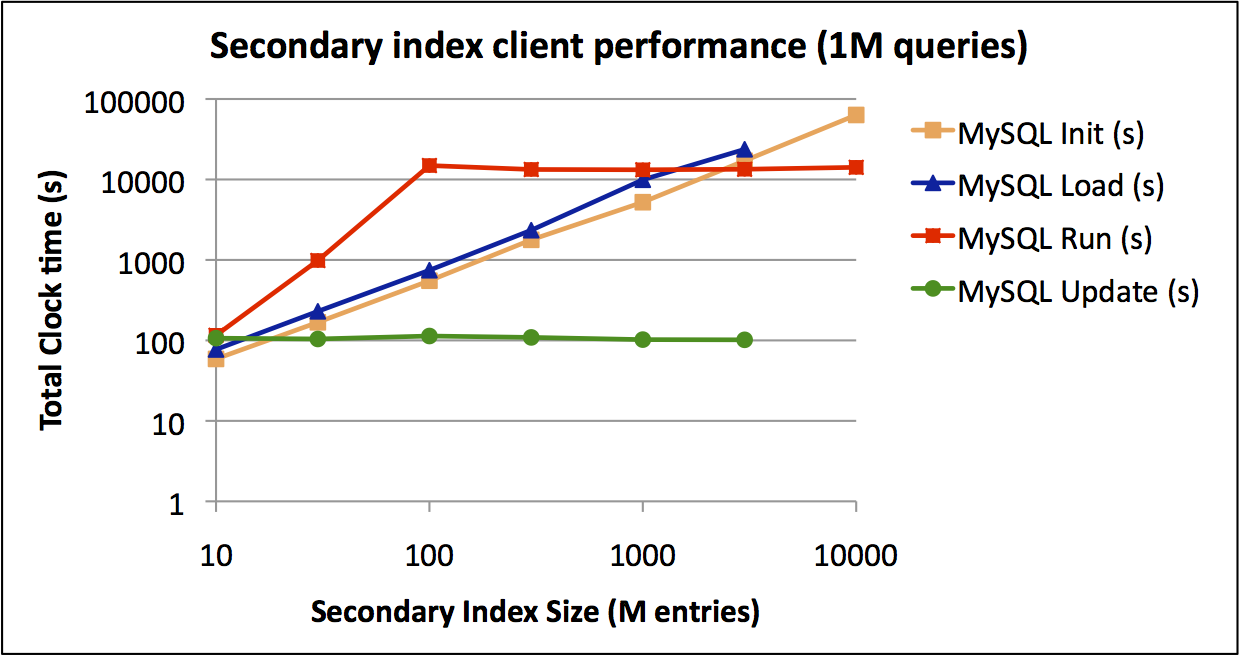
\includegraphics[width=\textwidth]{_static/indexing_tests.png}
\caption{Performance tests of MySQL-based secondary index. \label{fig:indexing-tests}}
\end{figure}

To improve the performance of the InnoDB storage engine for queries, the
secondary index may be split across a small number (dozens) of tables, each
containing a contiguous range of keys. This splitting, if done, will be
independent of the partitioning of the database itself. The contiguity of key
ranges will allow the secondary index service to identify the appropriate
split table arithmetically via an in-memory lookup.

\subsubsection{Secondary Index Structure}\label{secondary-index-structure}

The secondary index consists of three columns: the Object primary key
(objectId), the chunk where all data with that key are located (chunkId), and
the subchunk within that chunk where data with the key are located
(subChunkId). The objectId is assigned by the science pipelines as a 64-bit
integer value; the chunkId and subChunkId are both 16-bit integers which
identify spatial regions on the sky.

\subsubsection{Secondary Index Loading}\label{secondary-index-loading}

The InnoDB storage engine loads tables most efficiently if it is
provided input data which has been presorted according to the table's
primary key. When the secondary index information is collected for
loading (from each worker node handling a collection of chunks), it is
sorted by objectId, and may be divided into roughly equal ``splits''.
Each of those splits is loaded into a table \emph{en masse}.

To fully optimize the loading and table splitting, the entire index
should be collected from all workers and presorted in memory on the
master. This is not reasonable for 40 billion entries (requiring a minimum
of 480 GB memory, plus overhead). Instead, the index data from a single
worker can be assumed to be a ``representative sample'' from the full
range of objectIds, so table splitting can be done using the first
worker's index data. The remaining workers will be split and loaded
according to those defined tables.

\subsection{Data Distribution}\label{data-distribution}

LSST will maintain the released data store both on tape media and on a
database cluster. The tape archive is used for long-term archival. Three
copies of the compressed catalog data will be kept. The database cluster will
maintain 3 online copies of the data. Because computer clusters of reasonable
size failure regularly, the cluster must maintain replicas in order to provide
continuous data access. A replication factor of 3 is needed in order to
determine data integrity by majority rule when one replica is corrupt.

If periodic unplanned downtime is acceptable, an on-tape replica may
function as one of the three. However, the use of tape dramatically
increases the cost of recovering from a failure. This may be acceptable
for some tables, particularly those that are large and lesser-used,
although allowing service disruption may make it difficult to make
progress on long-running analysis on those large tables.

\subsubsection{Database data
distribution}\label{database-data-distribution}

The baseline database system will provide access for two database
releases: latest and previous . Data for each release will be spread out
among all nodes in the cluster.

Data releases are partitioned spatially, and spatial pieces (chunks) are
distributed in a round-robin fashion across all nodes. This means that
area queries involving multiple chunks are almost guaranteed to involve
resources on multiple nodes.

Each node should maintain at least 20\% free space of its data storage
allocation. The remaining free space is then available to be
``borrowed'' when another node fails. This will a temporary use of
storage capacity until more server resources can be put online, until
the 80\% storage use is returned.

\subsubsection{Failure and integrity
maintenance}\label{failure-and-integrity-maintenance}

There will be failures in any large cluster of node, in the nodes
themselves, in data storage volumes, in networks access and so on. These
failures will remove access to data that is resident on those nodes, but
this loss of data access should not affect that ability of scientists to
analyze the dataset as a whole. We need to set a data availability time
over 99.5\% to ensure confidence of the community in the stability of
the system. To ensure this level of data access, and to allow acceptable
levels of node failures in a cluster, there will be replication of data
on a table level throughout the cluster.

The replication level will be that each table in the database will exist
3 times, each on separate nodes. A monitoring layer to the system will
check on the availability of each table every few hours, although this
time will be tuned in practice. When this layer sees that a table has
less than three replicas available, this will initiate a replication of
that table to another nodes, not currently hosting that table. The times
for the checking, and speed of replication will be tuned to the
stability of the cluster, such that about 5\% of all tables at any given
time will only have 1 or 2 replicas. Three replicas will ensure that
tables will be available even in cases of large failures, or when nodes
need to be migrated to new hardware in bulk.

Should an entire node fail, replicating that data to another single node would
be fairly expensive in terms of time (on the order of hours).  We plan on
having free space on each node, filling local storage to 80\%. The free space
will be used for temporary storage of tables on failures, where replicas can
take place in parallel between nodes into this free space. When new nodes with
free storage are added to the cluster, then this data can be copied off this
free space into the drive, potentially taking several hours, but there will
still be 3 replicas of data during this time. Once this is complete, this data
will have 4 replicas for the short period of time until these tables can be
removed from the temporary storage, returning each node to 80\% usage.

\subsection{Metadata}\label{metadata}

Qserv needs to track various metadata information, static (not changing
or changing very infrequently), and dynamic (run-time) in order to
maintain schema and data integrity and optimize the cluster usage.

\subsubsection{Static metadata}\label{static-metadata}

Qserv typically works with databases and tables distributed across many
different machines: it breaks individual large tables into smaller chunks and
distributes them across many nodes. All chunks that belong to the same logical
table must have the same schema and partitioning parameters. Different tables
often need to be partitioned differently; for example some tables might be
partitioned with overlap (such as the Object table), some might be partitioned
with no overlap (for example the Source table), and some might not need
partitioning at all (e.g. a tiny Filter table). All this information about
schema and partitioning for all Qserv-managed databases and tables needs to be
tracked and kept consistent across the entire Qserv cluster.

Implementation of the static metadata in Qserv is based on hierarchical
key-value storage which uses a regular MySQL database as a storage
backend. This database is shared between multiple masters and it must be
served by a fault-tolerant MySQL server instance, e.g. using a
master-master replication solution like MariaDB Galera cluster. Database
consistency is critical for metadata and it should be implemented using
one of the transactional database engines in MySQL.

Static metadata may contain following information:

\begin{itemize}
\item
  Per-database and per-table partitioning and scan scheduling
  parameters.
\item
  Table schema for each table, used to create database tables in all
  worker and master instances; the schema in the master MySQL instance
  can be used to obtain the same information when a table is already
  created.
\item
  Database and table state information, used primarily by the process of
  database and table creation or deletion.
\item
  Definitions for the set of worker and master nodes in a cluster
  including their availability status.
\end{itemize}

The main clients of the static metadata are:

\begin{itemize}
\item
  Administration tools (command-line utilities and modules) which allow
  one to define or modify metadata structures.
\item
  Qserv master(s), mostly querying partitioning parameters but also
  allowed to modify table/database status when deleting/creating new
  tables and databases. Master(s) should not depend on node definitions
  in metadata; the XRootD facility is used to communicate with workers.
\item
  A special ``watcher'' service which implements distributed processes of
  database and table management.
\item
  An initial implementation of the data loading application which will
  use the node definitions and will create/update database and table
  definitions. This initial implementation will eventually be replaced
  by a distributed loading mechanism which may be based on separate
  mechanisms.
\end{itemize}

\subsubsection{Dynamic metadata}\label{dynamic-metadata}

In addition to static metadata, a Qserv cluster also needs to track its
current state, and keep various statistics about query execution. This
sort of data is updated frequently, several times per query execution,
and is called dynamic metadata.

The implementation of the dynamic metadata is based on the MySQL
database. Like static metadata it needs to be shared between all master
instances and is served via a single fault-tolerant MySQL instance
which is shared with static metadata database.

Dynamic metadata contains the following information:

\begin{itemize}
\item
  Definition of every master instance in a Qserv cluster.
\item
  Record of every SELECT-type query processed by cluster. This record
  includes query processing state and some statistical/timing
  information.
\item
  Per-query list of table names used by the asynchronous queries; this
  information is used to delay table deletion while async queries are in
  progress.
\item
  Per-query worker information, which includes chunk id and identifying
  information for the worker processing that chunk id. This information
  will be used to transparently restart the master or migrate query
  processing to a different master in case of master failure.
\end{itemize}

The most significant use of the dynamic metadata is to track execution
of asynchronous queries. When an async query is submitted it is
registered in the dynamic metadata and its ID is returned to the user
immediately. Later users can request status information for that query
ID which is obtained from dynamic metadata. When query processing is
finished, users can request results and the master can
obtain the location of the result data from dynamic metadata.

Additionally, dynamic metadata can be used to collect statistical
information about queries that were executed in the past which may be an
important tool in understanding and improving system performance.

\subsubsection{Architecture}\label{architecture}

The Qserv metadata system is implemented based on master/server
architecture: the metadata is centrally managed by a \emph{Qserv
Metadata Server} (qms). The information kept on each worker is kept to a
bare minimum: each worker only knows which databases it is supposed to
handle, and all remaining information can be fetched from the qms
as needed. This follows our philosophy of keeping the workers as
simple as possible.

The real-time metadata is managed inside qms in in-memory tables,
periodically synchronized with disk-based table. Such configuration
allows reducing qms latency -- important to avoid delaying query
execution time. Should a qms failure occur, the in-flight queries for
which the information was lost will be restarted. Since the
synchronization to disk-based table will occur relatively frequently
(e.g. at least once per minute), the lost time is insignificant. To avoid
overloading the qms, only the high-level information available from
Qserv-master is stored in qms; all worker-based information is cached in
a scratch space local to each worker in a simple, raw form (e.g,
key-value, ASCII file), and can be fetched on demand as needed.

\subsubsection{Typical Data Flow}\label{typical-data-flow}

Static metadata:

\begin{enumerate}
\def\labelenumi{\arabic{enumi}.}
\item
  Parts of the static metadata known before data is partitioned/loaded
  are loaded by the administration scripts responsible for loading data
  into the database, then these scripts start data partitioner.
\item
  The data partitioner reads static metadata loaded by the
  administration scripts, loads remaining information.
\item
  When Qserv starts, it fetches all static metadata and caches it in
  memory in a special, in-memory optimized C++ structure.
\item
  The contents of the in-memory metadata cache inside Qserv can be
  refreshed on demand if the static metadata changes (for example, when
  a new database or a table is added).
\end{enumerate}

Dynamic-metadata:

\begin{enumerate}
\def\labelenumi{\arabic{enumi}.}
\item
  Master loads the information for each query (when it starts, when it
  completes).
\item
  Detailed statistics are dumped by each worker into a scratch space
  kept locally. This information can be requested from each worker on
  demand. A typical use case: if all chunk-queries except one completed,
  qms would fetch statistics for the still-running chunk-query to
  estimate when the query might finish, whether to restart this query
  etc.
\end{enumerate}

\subsection{Shared Scans}\label{shared-scans}

Arbitrary full-table scanning queries must be supported in LSST's
baseline catalog, and in order to provide this support cost-effectively
and efficiently, Qserv implements shared scans. Shared scans effectively
reduce the I/O cost of executing multiple scanning queries
concurrently, reducing the require system hardware and purchasing costs.

Shared scans reduce overall I/O costs by forcing incoming queries to
share. When multiple queries scan the same table, theoretically, they
can completely share I/O and incur only the I/O cost of a single query
rather than the sum of their individual costs. In general, it is
difficult for queries to share I/O because their arrival times are
random and uncorrelated. Each query begins scanning at different times,
and because LSST's catalog tables will be so large, general system
caching is ineffective. In Qserv, scanning queries are broken up into
many parts, and shared scanning forces each query to operate on the same
portion of data at the same time by reordering and sequencing the query
fragments.

\subsubsection{Background}\label{shared-scan-background}

Historically, shared scanning has been a research topic that has very
few real-world implementations. We know of only one implementation in
use (Teradata). Most database implementations assume OS or database
caching is sufficient, encouraging heavy use of indexing to reduce the
need of table scans. However, our experiments have shown that when
tables are large enough (by row count) and column access sufficiently
variable (cannot index enough columns when there are hundreds to choose
from), indexes are insufficient. With large tables, indexes no longer
fit in memory, and even when they do fit in memory, the seek cost to
retrieve each row is dominant when the index selects a percentage of
rows, rather than some finite number (thousands or less).

\subsubsection{Implementation}\label{shared-scan-implementation}

The implementation of shared scans in Qserv is in two parts. The first
part is a basic classification of incoming queries as scanning queries
or non-scanning queries. A query is considered to scan a table if it
depends on non-indexed column values and involves more than \emph{k}
chunks (where \emph{k} is a tunable constant). Note that involving
multiple chunks implies that the query selects from at least one
partitioned table. This classification is performed during query
analysis on the front-end and leverages table metadata. The metadata
includes a ``scan rating'', which is set by hand. Higher scan ratings
indicate larger tables that take longer to read from disk. The
identified ``scan tables'' and their ratings are marked and passed along
to Qserv workers, which use the information in scheduling the fragments
of these scanning queries.

The second part of the shared scans implementation is a scheduling
algorithm that orders query fragment execution to optimize cache
effectiveness. Because Qserv relies on individual off-the-shelf DBMS
instances on worker nodes, it is not allowed to modify those instances
to implement shared scans. Instead, it issues query fragments ordered to
maximize locality of access in data and time, and tries to lock the
files associated with the tables in memory as much as possible. Using
the identified scan tables and their ratings, the worker places them on
the appropriate scheduler. There will be at least three schedulers. One
for queries expected to complete in under an hour, which are expected to
be related to the Object table. One for queries expected to take less
than eight hours, expected to be related to Object\_Extra. And one for
scans expected to take eight to twelve hours for ForcedSource and/or
Source tables. The reasoning being that a single slow query can impede
the progress of a shared scan and all the other user queries on that
scan. There may be a need for another scheduler to handle queries taking
more than 12 hours.

Each scheduler places incoming chunk queries into one of two priority
queues sorted by chunk id then scan rating of the individual tables. If
the query is for a chunk after the currently scanning chunk id, it is
placed on the active priority queue, otherwise it is placed on the
pending priority queue. After chunk id, the priority queue is sorted by
the table with highest scan rating to ensure that the largest tables in
the chunk are grouped together.

Once the query is on the appropriate scheduler, the algorithm proceeds
as follows: When a dispatch slot is available, it checks the highest
priority scheduler. If that scheduler has a query fragment (hereafter
called a task), and it is not at its quota limit, it is allowed to start
its next task, otherwise the worker checks the next scheduler. It
continues doing this until a task has been started or all the schedulers
have been checked.

Each scheduler is only allowed to start a task under certain circumstances.
There must be enough threads available from the pool so that none of the other
schedulers are starved for threads as well as enough memory available to lock
all the tables for the task in memory. If the scheduler has no tasks running,
it may start one task and have memory reserved for the tables in that task.
This should prevent any scheduler from hanging due to memory starvation
without requiring complicated logic, but it could incur extra disk I/O. More
on locking tables in memory later.

Schedulers check for tasks by first checking the top of the active
priority queue. If the active priority queue is empty, and the pending
priority queue is not, then the active and pending queues are swapped
with the task being taken from the top of the ``new'' active queue.

Since the queries are being run by a separate DBMS instance of which
there is little control over how it goes about running queries, the worker
can only control when queries are sent to the DBMS and also lock files in
memory. Files in memory are among the most likely items to be paged out
when memory resources are low, which would increase disk I/O. Locking
files in memory prevents this from happening. However, care must taken
in choosing how much memory can be used for locking files. Use too much
and there will be a significant impact on DBMS performance. Set aside
too little, and schedulers will not make optimum use of the resources
available and may be forced to run tasks without actually locking the
files in memory.

The memory manager controls which files are locked in memory. When a
scheduler tries to run a task, the task asks the memory manager to lock
all the shared scan tables it needs. The memory manager determines which
files are associated with the tables. If the files are already locked in
memory and there is enough memory available to lock the files which are
not already locked, the task is given a handle and allowed to run. When
the task completes, it hands the handle back to the memory manager. If
it was the last task using any particular table, the memory for the
files used by that table is freed.

When the memory manager locks a file, it does not read the file. It only
sets aside memory for the file to occupy when it is read by the DBMS. In
the special case where a task can run even though there is not enough
memory available, those tables that cannot fit are put on a list of
reserved tables and their size is subtracted from the quota until they
can be locked or freed. When memory is freed, the memory manager will
try to lock the reserved tables.

Because Qserv processes interactive, short queries concurrently with
scanning queries, its query scheduler should be able to allow for those
queries to complete without waiting for a query scan. To achieve this,
Qserv worker nodes choose between the scan scheduler described above and
a simpler \emph{grouping} scheduler. Incoming queries with identified
scan tables are admitted to the scan scheduler, and all other queries
are admitted to the grouping scheduler. The grouping scheduler is a
simple scheduler that is a simple variant of a plain FIFO
(first-in-first-out) scheduler. Like a FIFO scheduler, it maintains a
queue of queries to execute, and operates identically to a FIFO
scheduler with one exception -- queries are grouped by chunk id. Each
incoming query is inserted into the queue behind another query on the
same chunk, and at the back if no queued query matches. The grouping
scheduler assumes that the queue will never get very long, because it is
intended to only handle short interactive queries lasting fractions of
seconds, but groups its queue according to chunk id in order to provide
a minimal amount of access locality to improve throughput at a limited
cost to latency. Some longer queries will be admitted to the grouping
scheduler even though they are scanning queries, provided that they have
been determined to only scan a single chunk. Although these non-shared
scan query will disrupt performance of the overall scan on the
particular disk on a worker, the impact is thought to be small because
each of these represents all (or a large fraction of) the work for a
single user query, and the impact is amortized among all disks on all
workers.

For discussion about the performance of the existing prototype, refer
\citeds{DMTR-16}.

\subsubsection{Memory management}\label{shared-scan-memory-management}

To minimize system paging when multiple threads are scanning the same table,
we implemented a memory manager called memman. When a shared scan is about to
commence, the shared scan scheduler informs memman about the tables the query
will be using and how important it is to keep those tables in memory during
the course of the query. When directed to keep the tables in memory, memman
opens each data base table file, maps it into memory, and then locks the pages
to prevent the kernel from stealing the pages for other uses. Thus, once a
file page is faulted in, it stays in memory and allows other threads to scan
the contents of the page without incurring additional page faults. Once the
shared scan of the table completes, memman is told that the tables no longer
need to remain in memory. memman frees up the pages by unlocking them and
deleting the mapping.

This type of management is necessary to satisfy system paging requirements
because the prime paging pool is the set of unlocked file system pages.

\subsubsection{XRootD scheduling support}\label{shared-scan-xrootd-scheduling-support}

When the front-end dispatches a query, XRootD normally picks the least used
server in an attempt to spread the load across all of the nodes holding the
required table. While this works well for interactive queries, it is hardly
ideal for shared scan queries. In order to optimize memory and I/O usage,
queries for the same table in a shared scan should all be targeted to the same
node. A new scheduling mode was added to the XRootD cmsd called affinity
scheduling. The front-end can tell XRootD whether or not a particular query
has affinity to other queries using the same table. Queries that have affinity
are always sent to the same node relative to the table they will be using.
This allows the back-end scheduler to minimize paging by running the maximum
number of queries against the same table in parallel. Should that node fail,
XRootD assigns another working node that has the table as the target node for
queries that have affinity.

\subsubsection{Multiple tables support}\label{shared-scan-multiple-tables-support}

Handling multiple tables in shared scans requires an additional level of
management. The scheduler will aim to satisfy a throughput yielding average
scan latencies as follows:

\begin{itemize}
\item
  \texttt{Object} queries: 1 hour
\item
  \texttt{Object}, \texttt{Source} queries (join): 12 hours
\item
  \texttt{Object}, \texttt{ForcedSource} queries (join): 12 hours
\item
  \texttt{Object\_Extras}\footnote{This includes all
    \texttt{Object}-related tables, e.g., \texttt{Object\_Extra},
    \texttt{Object\_Periodic}, \texttt{Object\_NonPeriodic},
    \texttt{Object\_APMean}} queries (join): 8 hours.
\end{itemize}

There are be schedulers for queries that are expected to take one hour, eight
hours, or twelve hours. The schedulers group the the tasks by chunk id and
then the highest scan rating of the all tables in the task. The scan ratings
are meant to be unique per table and indicative of the size of the table, so
this sorting places scans using the largest table from the same chunk next to
each other in the queue. Using scan rating allows flexibility to work with
data sets with schemas different than that of LSST.

Since scans are not limited to specific tables, complicated joins could
occur in user queries that could take more than twelve hours to process.
The worker monitors query progress, and if particular queries appear to be
too slow for their current scheduler, they are removed and placed on a
dedicated "snail scan" so the rest of the queries on the original scheduler
are not overly delayed.

\subsection{Level 3: User Tables, External Data}\label{level-3-user-tables-external-data}

Level 3 tables including tables generated by users, and data catalogs
brought from outside, depending on their type and size, will be either
partitioned and distributed across the production database servers, or
kept unpartitioned in one central location. While the partitioned and
distributed Level 3 data will share the nodes with Level 2 data, it will
be kept on dedicated disks, independent from the disks serving Level 2
data. This will simplify maintenance and recoverability from failures.

Level 3 tables will be tracked and managed through the Qserv Metadata System
(qms), described in \secref{metadata}. This includes both the static, as well
as the dynamic metadata.

\subsection{Cluster and Task Management}\label{cluster-and-task-management}

Qserv delegates management of cluster nodes to XRootD. The XRootD system
manages cluster membership, node registration/deregistration, address lookup,
replication, and communication. Its Scalable Service Interface (SSI) API
provides data-addressed communication channels to the rest of Qserv, hiding
details like node count, the mapping of data to nodes, the existence of
replicas, and node failure. The Qserv master focuses on dispatching queries to
endpoints and Qserv workers focus on receiving and executing queries on their
local data.

Cluster management performed outside of XRootD does not directly affect query
execution, but includes coordinating data distribution, data loading, and node
arrival/departure, and is discussed in \secref{administration}. The SSI API
includes methods that allow dynamic updates to the data view of an XRootD
cluster so that when new tables appear or disappear, the XRootD system can
incorporate that information for future scheduling decisions. Thus, clusters
can dynamically change without the need to restart the XRootD system.

\subsection{Fault Tolerance}\label{fault-tolerance}

Qserv approaches fault tolerance in several ways. The design exploits the
immutability of the underlying data by replicating and distributing data
chunks across a cluster such that in the event of a node failure, the problem
can be isolated and all subsequent queries re-routed to nodes maintaining
duplicate data. Moreover, this architecture is fundamental to Qserv's
incremental scalability and parallel performance. Within individual nodes,
Qserv is highly modularized with minimal interdependence among its components,
which are connected via narrow interfaces. Finally, individual components
contain specialized logic for minimizing, handling, and recovering from
errors.

The components that comprise Qserv include features that independently provide
failure-prevention and failure-recovery capabilities. The MySQL proxy is
designed to balance its load among several underlying MySQL servers and
provide automatic fail-over in the event a server fails. The XRootD system
provides multiple managers and highly redundant servers to provide high
bandwidth, contend with high request rates, and cope with unreliable hardware.
And the Qserv master itself contains logic that works in conjunction with
XRootD to isolate and recover from worker-level failures.

A worker-level failure denotes any failure mode that can be confined to one or
more worker nodes. In principle, all such failures are recoverable given the
problem nodes are identified and alternative nodes containing duplicate data
are available. Examples of such failures include a disk failure, a worker
process or machine crashing, or network problems that render a worker
unreachable.

Consider the event of a disk failure. Qserv's worker logic is not equipped to
manage such a failure on localized regions of disk and would behave as if a
software fault had occurred. The worker process would therefore crash and all
chunk queries belonging to that worker would be lost. The in-flight queries on
its local mysqld would be cleaned up and have resources freed. The Qserv
master's requests to retrieve these chunk queries via XRootD would then return
an error code. The master responds by re-initializing the chunk queries and
re-submits them to XRootD. Ideally, duplicate data associated with the chunk
queries exists on other nodes. In this case, XRootD silently re-routes the
request(s) to the surviving node(s) and all associated queries are completed
as usual. In the event that duplicate data does not exist for one or more
chunk queries, XRootD would again return an error code. The master will re-
initialize and re-submit a chunk query a fixed number of times (determined by
a parameter within Qserv) before giving up, logging information about the
failure, and returning an error message to the user in response to the
associated query.

Error handling in the event that an arbitrary hardware or software bug
(perhaps within the Qserv worker itself) causes a worker process or machine to
crash proceeds in the same manner described above. The same is true in the
event that network loss or transient sluggishness/overload has the limited
effect of preventing XRootD from communicating with one or more worker nodes.
As long as such failures are limited to a finite number of workers and do not
extend to the Qserv master node, XRootD is designed to record the failure and
return an error code. Moreover, if duplicate data exists on other nodes, this
will be registered within XRootD, which will successfully route any subsequent
chunk queries.

In the event of an unrecoverable error, the Qserv master is equipped with a
status/error messaging mechanism designed to both log detailed information
about the failure and to return a human-readable error message to the user.
This mechanism includes C++ exception handling logic that encapsulates all of
the master's interactions with XRootD. If an unrecoverable exception occurs,
the master gracefully terminates the query, frees associated resources, logs
the event, and notifies the user. Qserv's internal status/error messaging
system also generates a status message and timestamp each time an individual
chunk query achieves a milestone. Such milestones include: chunk query
dispatch, written to XRootD, results read from XRootD, results merged, and
query finalized. This real-time status information provides useful context in
the event of an unrecoverable error.

Building upon the existing fault-tolerance and error handling features
described above, future work includes introducing a heartbeat mechanism on
worker nodes that periodically pings the worker process and will restart it in
the event it becomes unresponsive. Similarly, a master monitoring process
could periodically ping worker nodes and restart a worker machine if
necessary. We are also considering managing failure at a per-disk level, but
this would require research since application-level treatment of disk failure
is relatively rare. It should also be possible to develop an interface for
checking the real-time status of queries currently being processed by Qserv by
leveraging its internally used status/error messaging mechanism.

\subsection{Next-to-database Processing}\label{next-to-database-processing}

We expect some data analyses will be very difficult, or even impossible to
express through SQL language. This might be particularly useful for time-
series analysis. For this type of analyses, we will allow users to execute
their analysis algorithms in a procedural language, such as Python. To do
that, we will allow users to run their own code on their own hardware
resources co-located with production database servers. Users then run queries
on the production database which stream rows directly from database cluster
nodes to the user processing cluster, where arbitrary code may run without
endangering the production database. This allows their incurred database I/O
needs to be satisfied using the database system's shared scanning
infrastructure while providing the full flexibility of running arbitrary code.

\subsection{Administration}\label{administration}

\subsubsection{Installation}\label{installation}

Qserv as a service requires a number of components that all need to be
running, and configured together. On the master node we require mysqld, mysql-
proxy, XRootD, cmsd, Qserv metadata service, and the Qserv master process. On
each of the worker nodes there will also be the mysqld, cmsd, and XRootD
service. These major components come from the MySQL, XRootD, and Qserv
distributions. But to get these to work together we also require many more
software package, such as protobuf, Lua, expat, libevent, python, zope, boost,
Java, antlr, and so on. And many of these require more recent versions than
are provided in most system distributions.

To manage both the complexity of deployment and the diversity of possible
installation environments, we have adopted the use of Linux containers via
Docker.  Service binaries and their user-space dependencies are bundled within
containers which can then be deployed uniformly to any host running Docker
with a recent enough Linux kernel, regardless of operating system
distribution, package profile, patch levels, etc.

We have experimented with several container orchestration technologies
during development.  Of these, Kubernetes seems to be emerging as a clear
leader, and is our current orchestration solution of choice.

\subsubsection{Data loading}\label{data-loading}

As previously mentioned, Data Release Production will not write directly
to the database. Instead, the DRP pipelines will produce binary FITS
tables and image files that are reliably archived as they are produced.
Data will be loaded into Qserv in bulk for every table, so that tables
are either not available, or complete and immutable from the user query
access perspective.

For replicated tables, these FITS files are converted to CSV (e.g. by
harvesting FITS image header keyword value pairs, or by translating
binary tables to ASCII), and the resulting CSV files are loaded directly
into MySQL and indexed. For partitioned tables like Object and Source,
FITS tables are fed to the Qserv partitioner, which assigns partitions
based on sky coordinates and converts to CSV.

In particular, the partitioner divides the celestial sphere into
latitude angle ``stripes'' of fixed height H. For each stripe, a width W
is computed such that any two points in the stripe with longitudes
separated by at least W have angular separation of at least H. The
stripe is then broken into an integral number of chunks of width at
least W, so that each stripe contains a varying number of chunks (e.g.
polar stripes will contain just a single chunk). Chunk area varies by a
factor of about pi over the sphere. The same procedure is used to obtain
subchunks: each stripe is broken into a configurable number of
equal-height ``substripes'', and each substripe is broken into
equal-width subchunks. This scheme is preferred over the Hierarchical
Triangular Mesh for its speed (no trigonometry is required to locate the
partition of a point given in spherical coordinates), simplicity of
implementation, and the relatively fine control it offers over the area
of chunks and sub-chunks.

The boundaries of subchunks constructed as described are boxes in
longitude and latitude - the overlap region for a subchunk is defined as
the spherical box containing all points outside the subchunk but within
the overlap radius of its boundary.

The task of the partitioner is to find the IDs of the chunk and subchunk
containing the partitioning position of each row, and to store each row
in the output CSV file corresponding to its chunk. If the partitioning
parameters include overlap, then the row's partitioning position might
additionally fall inside the overlap regions of one or more subchunks.
In this case, a copy of the row is stored for each such subchunk (in
overlap CSV files).

Tables that are partitioned in Qserv must be partitioned identically
within a Qserv database. This means that chunk tables in a database
share identical partition boundaries and identical mappings of chunk id
to spatial partition. In order to facilitate table joining, a single
table's columns are chosen to define the partitioning space and all
partitioned tables (within a related set of tables) are either
partitioned according that pair of columns, or not partitioned at all.
Our current plan chooses the Object table's \texttt{ra\_PS} and
\texttt{decl\_PS} columns, meaning that rows in the Source and
ForcedSource tables will be partitioned according to the Objects they
reference.

There is one exception: we allow for precomputed spatial match tables.
As an example, such a table might provide a many-to-many relationship
between the LSST Object catalog and a reference catalog from another
survey, listing all pairs of LSST Objects and reference objects
separated by less than some fixed angle. The reference catalog cannot be
partitioned by associated Object, as more than one Object might be
matched to a reference object. Instead, the reference catalog must be
partitioned by reference object position. This means that a row in the
match table might refer to an Object and reference object assigned to
different chunks stored on different Qserv worker nodes.

We avoid this complication by again exploiting overlap. We mandate (and
verify at partitioning time) that no match pair is separated by more
than the overlap radius. When partitioning match tables, we store a copy
of each match in the chunk of both positions referenced by that match.
When joining Objects to reference objects via the match table then, we
are guaranteed to find all matches to Objects in chunk C by joining with
all match records in C and all reference objects in C or in the overlap
region of C.

All Qserv worker nodes will partition subsets of the pipeline output
files in parallel -- we expect partitioning to achieve similar aggregate
I/O rates to those of full table scans for user query access, so that
partitioning should complete in a low factor (2-3x) of the table scan
time. Once it does, each Qserv worker will gather all output CSV files
for its chunks and load them into MySQL. The structure of the resulting
chunk tables is then optimized to maximize performance of user query
access (chunk tables will likely be sorted, and will certainly be
compressed), and appropriate indexes are built. Since chunks are sized
to fit in memory, all of these steps can be performed using an in-memory
file-system. I/O costs are incurred only when reading the CSV files
during the load and when copying finalized tables (i.e. .MYD/.MYI files)
to local disk.

The last phase of data loading is to replicate each chunk to one other
Qserv worker node. We will rely on table checksum verification rather
than a majority rule to determine whether a replica is corrupt or not.

The partitioner has been prototyped as a multi-threaded C++ program. It
uses an in-memory map-reduce implementation internally to scale across
cores, and can read blocks of one or more input CSV files in parallel.
It does not currently understand FITS table files. CSV file writes are
also parallelized - each output chunk is processed by a single reducer
thread and can be written to in parallel with no application level
locking. In preliminary testing, our partitioner was able to sustain
several hundred MB/s of both read and write bandwidth when processing a
CSV dump of the PT1.2 Source table.

We are investigating a pair of data loading optimizations. One is to
have pipeline processes either integrate the partitioning code or feed
data directly to the partitioner, rather than communicating via
persistent storage. The other is to write out tables in the native
database format (e.g. as .MYD files, ideally using the MySQL/MariaDB
server code to do so), allowing the CSV database loading step to be
bypassed.

\subsubsection{Administrative scripts}\label{administrative-scripts}

The Qserv design originally had a somewhat complicated set of custom scripts
and tools used to coordinate and sequence service launch and shutdown on a
cluster, to monitor and report on service status, to automatically relaunch
failed services, and to coordinate rolling software upgrades out onto a
cluster.  We have recently found that all of these needs are directly met by
container orchestration frameworks such as Kubernetes, and so we are currently
in to process of removing this now-redundant tooling in order to simplify and
standardize the design.

Data ingest still tends to be a slightly detailed process, beyond just data
preparation. Up to now, data preparation produces text files in CSV format
which are then loaded into the MySQL layer as a MyISAM table. The schema for
these tables then needs to be elaborated in places with columns for chunk and
subchunk number.  Loading is done with index-creation suspended, and indices
and table statistics for the query planner need to be explicitly generated
on each worker after the load.  Additionally, a list of chunks on the sky
for which no data has been loaded must be generated to aid in efficient
query dispatch.  All of these activities are currently coordinated by a
Python qserv-loader script.

\subsection{Current Status and Future
Plans}\label{current-status-and-future-plans}

As of now (July 2017) we have implemented a basic version of Qserv end-to-end,
and maintain three running instances at a scale of approximately 30 physical
nodes each in continuous operation on dedicated hardware clusters at NCSA and
CC-IN2P3.

The system has been demonstrated to correctly distribute and execute both low
and high volume queries, including small-area cone and object searches, region
restricted queries, and full table scans including large-area near-neighbor
searches.  Analytic queries involving SciSQL UDFs in both filter and
aggregation clauses have also been demonstrated.

Scale testing has been successfully conducted \footnote{See Qserv test reports
\citeds{DMTR-21}, \citeds{DMTR-12}, \citeds{DMTR-13}, and \citeds{DMTR-16}
(most recent).} on the above-mentioned clusters with datasets of up to
approximately 70 TB, and we expect to cross the 100 TB mark as tests continue
in 2017.  To date the system is on track through a series of graduated data-
challenge style tests \citedsp{LDM-552} to meet or exceed the stated
performance requirements for the project \citedsp{LDM-555}.

The shared-scan implementation is substantially complete, and functions per
design to enable high levels of concurrency without degraded full-scan query
performance.

The metadata system, as described above, for both static and dynamic metadata
is in place, and basic query management facilities (query cancellation and
monitoring) have been implemented.

The system includes a comprehensive set of unit and regression tests that are
integrated with the build and CI systems.

In addition to background ongoing effort to improve query performance and
extend query coverage, implementation work ahead includes:

\begin{itemize}
\item
  automatic data distribution and replication;
\item
  improved query management and monitoring tools;
\item
  demonstrating cross-match with external catalogs;
\item
  implementing support for Level 3 data;
\item
  next-to-data processing framework;
\item
  improvements to administration procedures and scripts;
\item
  authentication and authorization;
\item
  resource management;
\item
  security.
\end{itemize}

\textbf{Automatic data distribution and replication}. We have experimented
successfully with static replication of data at ingest time, but for
production a system which will automatically place data and dynamically
respond dynamically to node arrivals and departures will be required.
This is currently under active development.

\textbf{Improved query management and monitoring tools}. The facility to
enable clients to temporarily disconnect from long-running queries and later
rendezvous to check query progress and/or collect results is currently under
active development.  Facilities to return partial results and estimate
completion times and data sizes for long-running queries remain to be
implemented.

\textbf{Demonstrating cross-match with external catalogs}. One of the use
cases involves cross matching with external catalogs. In cases where the
catalog to cross-match with is small, it will be replicated. For
cross-matching with larger catalogs, the catalog to be cross-matched with
will need to be partitioned and distributed to the worker nodes.

\textbf{Implementing support for Level 3 data}. Users should be able to
maintain their own tables to store their own data or results from previous
queries. They should be able to create, drop, and replace their own tables
within the system.

\textbf{Next to data processing framework}. A facility to stream query
results to dedicated nodes where user-submitted code can run against
those streams has yet to be implemented.

\textbf{Improvements to administration procedures and scripts}. To further
automate common tasks related to database management, table management,
partition management, data distribution, and others we need to implement
various  improvements to our administration procedures and scripts.

\textbf{Authentication and authorization}. A production database system should
provide some facility for user or role-based access so that usage can be
controlled and resources can be shared. This is in particular needed for
Level-3 data products.

\textbf{Resource management}. A production system should have some way
to manage/restrict resource usage and provide quality-of-service
controls. This includes a monitoring facility that can track each node's
load and per-user-query resource usage.

\textbf{Security}. The system needs to be secure and resilient against
denial of service attacks.

\subsection{Open Issues}\label{open-issues}

What follows is a (non-exhaustive) list of issues, technical and scientific,
that are still being discussed and where changes are possible.

\begin{itemize}
\item
  \textbf{Row updates}. Currently, all rows once ingested into a Qserv
  instance are treated as immutable, and row updates are not supported. This
  simplification of design is possible because the motivating use case for
  Qserv (annually released, authoritative, LSST catalogs) is primarily
  read-only.  The apparent need for update of Level 3 products within a Qserv
  instance can be worked around by treating Level 3 products as immutable once
  ingested; should changes to a Level 3 product be required, that product
  would be dropped and re-ingested/regenerated rather than updated in place.
  If it were deemed necessary that Qserv support row updates and/or
  transactions directly, some considerable changes to the Qserv architecture
  would likely be required.
\item
  \textbf{Very large objects}. Some objects (e.g. large galaxies) are
  much larger than our overlap region; in some cases their footprint
  will span multiple chunks. Currently we are working with the object
  center, neglecting the actual footprint. While there are some science
  use cases that would benefit from a system that tracks objects based
  on their footprint, this is currently not a requirement. A potential
  solution would involve adding a custom index similar to the
  r-tree-based indexes such as the TOUCH
  \citep{Nobari:2013:TIS:2463676.2463700}.
\item
  \textbf{Very large results}. Currently, the front-end that dispatches
  a query is also responsible for assembling its eventual results. In general,
  this is not a scalable approach as the resources required to processes the
  results may be several orders of magnitude greater than those needed
  to dispatch the query.  One potential solution is to replicate the
  front-end to the extent necessary to handle query results. Alternatively,
  the XRootD SSI interface could be augmented to itself allow running
  disconnected queries. That is, once a particular front-end dispatches
  a query it can get a handle to that query and disconnect from it.
  A different server could, using that handle, reconnect to the query and
  process the results. This would be a more flexible model as it would allows
  independent scaling of query dispatch and result processing. It would also
  have the benefit of not requiring cancellation of in-progress queries
  dispatched from a particular front-end should that front-end die.
\item
  \textbf{Sub-queries}. Qserv does not currently support SQL sub-queries.
  Since there is evidence that such a capability might be useful to users, we
  should formulate a few possible designs and understand how easy/difficult
  they might be to implement.  Some potential approaches here might be to
  split sub-queries into multiple queries and/or use session variables. A
  naïve implementation that involves dumping all sub-query results to disk
  and then rereading them, similar to a multi-stage map/reduce, should also
  be tractable.
\end{itemize}

\section{Risk Analysis}\label{risk-analysis}

\subsection{Potential Key Risks}\label{potential-key-risks}

Insufficient \textbf{database performance and scalability} is one of the
major stated major risks for DM \citedsp{Document-7025}.

Qserv as an implementation of the baseline architecture meeting the
requirements referenced above is already well on its way, and is currently
resourced and scheduled for completion on time and within budget.

A viable alternative might be to use an off-the-shelf system. In fact, an off-
the-shelf solution could present significant support cost advantages over a
production-ready Qserv, especially if it is a system well supported by a large
user and developer community. It is likely that an open source, scalable
solution will be available on the time scale needed by LSST (for the beginning
of production scalability approaching few hundred terabytes would be
sufficient). Database systems larger than the largest single LSST data set
have been successfully demonstrated in production today.  There is a growing
demand for large scale systems and growing competition in that area (Hadoop,
Greenplum, InfiniDB, MonetDB, Caché and others).  Greenplum, which was a
closed-source project at the outset of LSST, is now available as open-source.

Finally, a third alternative would be to use a closed-source, non free
software, such as Caché or InfiniDB (Teradata is too expensive). Some of these
systems are very reasonably priced. We believe the largest barrier preventing
us from using an off-the-shelf DBMS such as InfiniDB is poorly developed
spherical geometry and spherical partitioning support.

Potential \textbf{problems with off-the-shelf database software} used,
such as MySQL is another potential risk. MySQL has recently been
purchased by Oracle, leading to doubts as to whether the MySQL project
will be sufficiently supported in the long-term. Since the purchase,
several independent forks of MySQL software have emerged, including
MariaDB (supported by one of the MySQL founders) and Percona. Should MySQL disappear, these open-source,
MySQL-compatible systems are a solid alternative. Should we need to
migrate to a different DBMS, we have taken multiple measures to minimize
the impact:

\begin{itemize}
\item
  our schema does not contain any MySQL-specific elements and we have
  successfully demonstrated using it in other systems such as MonetDB;
\item
  we do not rely on any MySQL specific extensions, with the exception of
  MySQL Proxy, which can be made to work with non-MySQL systems if
  needed;
\item
  we minimize the use of stored functions and stored procedures which
  tend to be DBMS-specific, and instead use user defined functions,
  which are easier to port (only the interface binding part needs to be
  migrated).
\end{itemize}

\textbf{Complex data analysis}. The most complex analysis we identified
so far include spatial and temporal correlations which exhibit
\(O(n^2)\) performance characteristics, searching for anomalies and rare
events, as well as searching for unknown are a risk as well -- in most
cases industrial users deal with much simpler, well defined access
patterns. Also, some analysis will be ad-hoc, and access patterns might
be different than these we are anticipating. Recently, large-scale
industrial users have started to express strong need for similar types of
analyses; understanding and correlating user behavior (time-series of
user clicks) run by web companies, searching for abnormal user behavior
to detect fraud activities run by banks and web companies, analyzing
genome sequencing data run by biotech companies, and what-if market
analysis run by financial companies are just a few examples. Typically
these analyses are ad-hoc and involve searching for unknowns, similar to
scientific analyses. As the demand (by rich, industrial users) for this
type of complex analyses grows, the solution providers are rapidly
starting to add needed features into their systems.

The complete list of all database-related risks maintained in the LSST
risk registry:

\begin{itemize}
\item
  DM-014: Database performance insufficient for planned load
\item
  DM-015: Unexpected database access patterns from science users
\item
  DM-016: Unexpected database access patterns from DM productions
\item
  DM-032: LSST DM hardware architecture becomes antiquated
\item
  DM-060: Dependencies on external software packages
\item
  DM-061: Provenance capture inadequate
\item
  DM-065: LSST DM software architecture incompatible with de facto
  community standards
\item
  DM-070: Archive sizing inadequate
\item
  DM-074: LSST DM software architecture becomes antiquated
\item
  DM-075: New SRD requirements require new DM functionality
\end{itemize}

\subsection{Risks Mitigations}\label{risks-mitigations}

To mitigate the insufficient performance/scalability risk, we developed Qserv,
and demonstrated scalability and performance. In addition, to increase chances
an equivalent open-source, community supported, off-the-shelf database system
becomes available we have closely collaborated with the MonetDB open source
columnar database team -- building on our Qserv lessons-learned, they are
trying to add missing features and turn their software into a system capable
of supporting LSST needs. Further, to stay current with the state-of-the-art
in petascale data management and analysis, we continue a dialog with all
relevant solution providers, both DBMS and Map/Reduce, as well as with data-
intensive users, both industrial and scientific, through the XLDB conference
and workshop series we lead, and beyond.

To understand query complexity and expected access patterns, we are
working with LSST Science Collaborations and the LSST Science Council to
understand the expected query load and query complexity. We have
compiled a set of common queries \citep{CommonQueries} and distilled
this set into a smaller set of representative queries we use for various
scalability tests -- this set represents each major query type, ranging
from trivial low volume, to complex correlations \citep{PerfTests}. We
have also talked to scientists and database developers from other
astronomical surveys, including SDSS, 2MASS, Gaia, DES, LOFAR and
Pan-STARRS.

To deal with unpredictability of analysis, we will use shared scans.
With shared scans, users will have access to all the data, all the
columns, even these very infrequently used, at a predictable cost --
with shared scans increasing complexity does not increase the expensive
disk I/O needs, it only increases the CPU needs.

To keep query load under control, we will employ throttling to limit
individual query loads.

\section{References}\label{references}
\renewcommand{\refname}{}
\bibliography{local,lsst,lsst-dm,refs_ads,refs,books}

\end{document}
